\documentclass{article}
\usepackage[%
    left=0.5in,%
    right=0.5in,%
    top=0.5in,%
    bottom=0.5in,%
]{geometry}%
\usepackage{minitoc}
\usepackage{mathtools}
\usepackage{multicol}
\usepackage{graphicx}
\usepackage{amssymb}
\usepackage{fixltx2e}
\usepackage{listings}
\usepackage{color}
\usepackage{hyperref}
    \hypersetup{ colorlinks = true, linkcolor = blue }
\usepackage{blindtext}
\definecolor{lightgray}{gray}{0.9}
\graphicspath{ {./} }
\usepackage{stmaryrd}

\newcommand\Hoaretriple[3]{%
  \llparenthesis\,#1\,\rrparenthesis
  \mathrel{#2}\nolinebreak 
  \llparenthesis\,#3\,\rrparenthesis
}

\begin{document}
\section{Loop invariant}
\begin{center}
  \makebox[\textwidth]{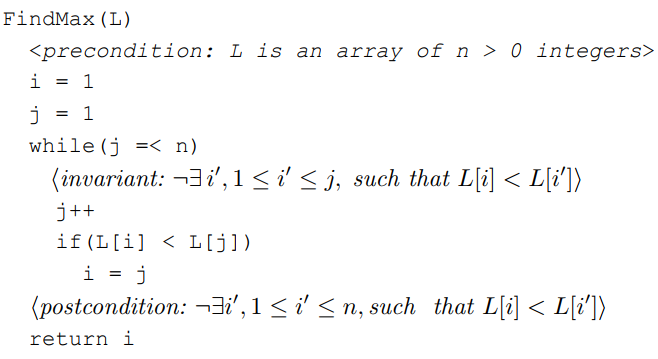
\includegraphics[scale=0.5]{Selection_022.png}}
\end{center}

\begin{flushleft}
To establish a loop invariant we need to show two things:
\begin{itemize}
	\item \textbf{initialisation}: The invariant is true prior to the first iteration of the loop
	\item \textbf{maintenance}: If the invariant is true before an iteration of the loop, it remains true in the next iteration
\end{itemize}
If those two properties hold, the invariant is true prior to every iteration of the loop and when the loop terminates. Typically we'd use code in the loop body to prove that the invariant remains true before each iteration.
\end{flushleft}

\subsection{Proving partial correctness using while}
\begin{flushleft}
To use the while rule ina proof of correctness of \textit{FindMax}
\[
\psi \: \text{is} \:  \neg \exists \text{i',} 1 \leqslant \text{i'} \leqslant j \: \text{such that} \: L[\,i]\, < L[\, \text{i'} ]\,
\]
\[ B \:\text{is}\: j \leqslant n \: \text{and} \: \neg B \:\text{is}\: j \nleq n \]
B holds because of precondition $n > 0$ and $j$ is initialised to 1. So provided the loop therminates $\psi$ and $\neg B$ together imply that
\[
\neg \exists \text{i',} 1 \leqslant \text{i'} \leqslant n \: \text{such that} \: L[\,i]\, < L[\, \text{i'} ]\,
\]
The loop invariants can be used to prove partial correctness. An algorithm that produces the desired output for all inputs \textbf{when the algorithm terminates} is said to be \textit{partially correct}.\\
To prove total correctness we need an algorithm that is \textit{partially correct} and is \textbf{guaranteed to terminate}.
\end{flushleft}
\end{document}
